\section{Origin}
Because this project is about shaping the directional characteristics of loudspeakers arrangements towards a particular direction, it is important to thorougly investigate the directional characteristic of a single loudspeaker cabinet. This serves as a baseline for comparison and also is essential, because the investigated cabinet will be used to form the speaker array later on.\\
In general, loudspeakers tend to display different directional behaviour depending on the frequency emitted. At low frequencies they can be viewed as omnidirectional sound sources. At higher frequencies the main direction of sound emission is in line with the motion direction of the voice coil. \citep[p. 910 f.]{crocker98}
Depending on the ratio of the emitted wavelength to the diameter of the speaker, a radiation pattern with side lobes can occur. An analytic approximation to the behaviour can be made  when looking at a vibrating piston in an infinite baffel. However, this only takes into account the front side of the speaker. It is difficult to incorporate the effects of an enclosure into this model.\\
There are possibilities to numerically model the sound field around a speaker in a cabinet. However in the context of this project, conducting a measurement seems to be the most favourable approach towards quantifying the sound pressure emitted by loudspeaker mounted in an enclosure. Measurements must be taken at numerous frequencies and positions along a circular trajectory.
For this project, measurements are conducted by placing the test object on a turntable in free field conditions and measuring transfer functions with a microphone. The voltage output of the amplifier and the gain of the microphone can be calibrated so that the only part unknown is transduction performed by the test object.
The knowledge gained through these measurements can then be used in order to designate a feasible frequency range for beamforming in the way that will be described later on. 

\section{Transfer Function Measurement with Sweeps}\label{sec:sweep_theorie}
The characterization of the directional behaviour of the speaker consists of a large number of transfer function measurements. While there are many methods available to obtain transfer functions, it was decided to go with a method that is based on sweeps, due to several benefits. \citep[p. 3 ff.]{mueller01}\\
The sweep signal used for the measurement can be generated by the \gls{ift} of a desired spectrum and a group delay that is designed accordingly. This results in a sinusidal waveform with a continuously altering frequency. In most cases it is desirable to keep a nearly constant amplitude over the whole length of the sweep. The procedure of generating such a sweep signal is illustrated in \autoref{fig:sweep_signal}.

\begin{figure}[htbp]
	\centering
	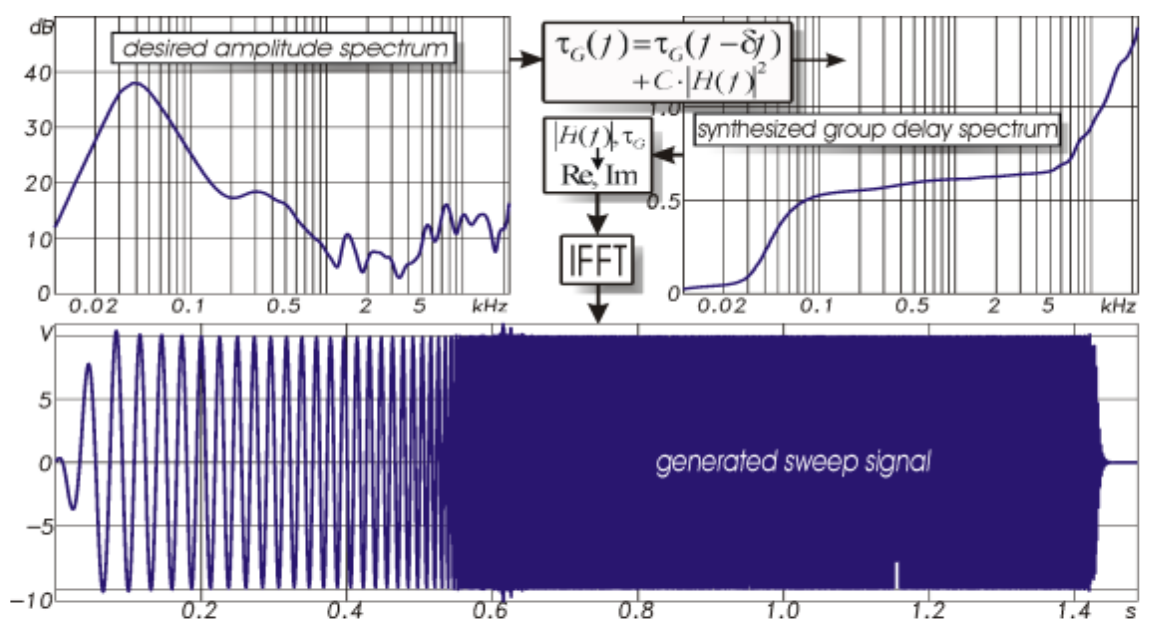
\includegraphics[width=1\textwidth]{mueller01_sweep.png}
	\caption{Sweep synthesis with arbitrary spectral magnitude and nearly constant envelope, taken from \citep{mueller01}}
		\label{fig:sweep_signal}
\end{figure}

The test signal is played back via the loudspeaker that is the test object and the sound is recorded with a microphone in a particular angle towards the main axis of the loudspeaker. An \gls{fft} is performed on the recorded signal. The transfer function of the loudspeaker is then calculated by a multiplication operation with the recorded signal and the inverse of the test signal in frequency domain. It has to be taken into account, that not only the properties of the loudspeaker, but also the distance between the loudspeaker and the microphone and the sound field in the room have an influence on the measurement results. In the context of this project is therefore expedient to conduct the measurements in free field conditions, which means resorting to an anechoic chamber.\\
One particular advantage of sweep measurements over other methods to determine the transfer function is that nonlinearities in the measurement chain or the test object, that lead to distortion, can be isolated from the measured transfer function and can be assessed seperately. \citep[p. 20 f.]{mueller01} Simply put, this property is due to the face, that in the sweep signal, every frequency has a certain group delay, which leads to harmonics being displayed at a negative time when the test signal and the measured signal are convolved in time domain. While it is not the subject of this project to investigate nonlinearities in the behaviour of the speaker in depth, keeping track of the distortion helps with keeping the gains in the measurement chain at a good operating level.

\section{Measurement Setup}\label{sec:meas_setup}
In order to obtain the data that is required for making polar plots at several frequencies or isobar diagrams, the transfer functions have to be measured at numerous points. To make measurements more time efficient the loudspeaker is placed on a turntable. The acoustical center (see also \autoref{sec:ac_center}) the loudspeaker is placed on the turning axis. The gain on the microphone amplifier and the input of the soundcard are calibrated, so that a known digital value at the soundcard corresponds to a known sound pressure at the microphone membrane. The gain of the power amplifier that drives the speaker is adjusted, so that a known value at the output of the soundcard corresponds to a known voltage over the terminals of the speaker. With these prerequesits the transfer function can be quantified as sound pressure per voltage at a given distance. The rotation of the turntable, on which the loudspeaker is placed, is controlled by the measurement routine on the computer. After every transfer function measurement, the orientation of the loudspeaker is altered, so that the measurement angles are evenly distributed along the circumference. The measurement data are stored, so that they can be processed into a readable form subsequently.


\begin{figure}[htbp]
	\centering
\begin{picture}(0,0)%
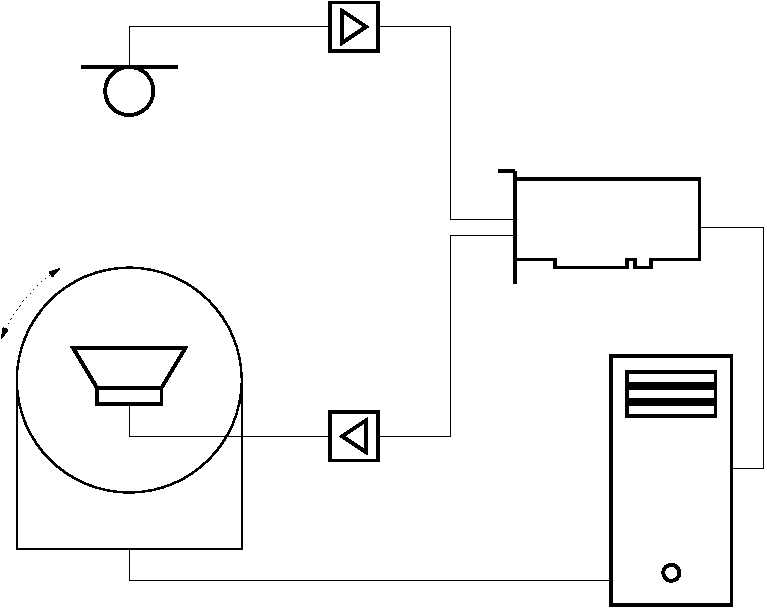
\includegraphics{meas_setup_01.pdf}%
\end{picture}%
\setlength{\unitlength}{2818sp}%
\begingroup\makeatletter\ifx\SetFigFont\undefined%
\gdef\SetFigFont#1#2#3#4#5{%
  \reset@font\fontsize{#1}{#2pt}%
  \fontfamily{#3}\fontseries{#4}\fontshape{#5}%
  \selectfont}%
\fi\endgroup%
\begin{picture}(8570,6816)(3053,-7474)
\put(4900,-1771){Microphone}%
\put(6525,-1501){Amplifier}%
\put(3250,-7081){Turntable}%
\put(6525,-6091){Amplifier}%
\put(9125,-3211){Sound Card}%
\put(10025,-6361){Computer}%
\end{picture}%
\caption{Measurement setup for transfer functions; for convenience the loudspeaker is placed on a turntable, that is controlled by the measurement routine on the computer.}
\label{fig:measurement_setup}
\end{figure}

\section{Determining the Acoustical Center of the Test Object}\label{sec:ac_center}
In order to achieve meaningful results regarding the directional characteristic of the a loudspeaker, it is necessary to know the location of the  acoustical center of the loudspeaker.
In \citep{ansis1.1}, the ``effective acoustical center'' of an electroacoustical transducer is defined as the ``position of the effective or virtual point source from which sound pressure varies inversely as distance''. This concept is further discussed in \citep{jacobsenetal}, where the authors also state, that the position of the acoustic center is frequency dependent. For gathering the data to characterize the directivity it is desirable to position the acoustic center of the \gls{dut} on the rotational axis of the turntable. This can lead to practical difficulties due to the frequency dependency. It is therefore necessary to assess the position of the acoustical center of the \gls{dut} in the desired frequency range via a measurement.

%A way to determine the acoustical center by measurement can be proposed as follows. The loudspeaker is placed on the turntable, oriented with its main axis directly towards the measurement microphone (\SI{0}{\degree}). Details about this procedure can be found in \autoref{ax:directional_1}.






\section{The beamwidth of the \gls{dut}}\label{sec:ac_center}
In order to find the beamwidth of the \gls{dut}, a pre polar response measurement have to be done to localize the acoustic center of the \gls{dut} by analyse the polar phase of the \gls{dut}. With the knowledge of the polar phase to a given frequency, it is possible to calculate the distance in x and y direction, the \gls{dut} have to be moved. The pre polar response is explained in \autoref{ax:directional_1}, and in \autoref{} the moment was calculated to ... in x direction and ... in y direction. 
After the speaker is moved to the calculated position, the polar response is measured again and analysed in \autoref{ax:directional_2}. Because of flexibility of the first stand in \autoref{ax:directional_1}, the position of the speaker is of with \SI{4.5}{\centi\meter} to the front. The measurement  is executed according to \autoref{appendix:beamwidth} and the beamwidth of the \gls{dut} is as following \autoref{fig:beamwidth_offset_4.5_cm} 

\begin{figure}[htbp]
	\centering
	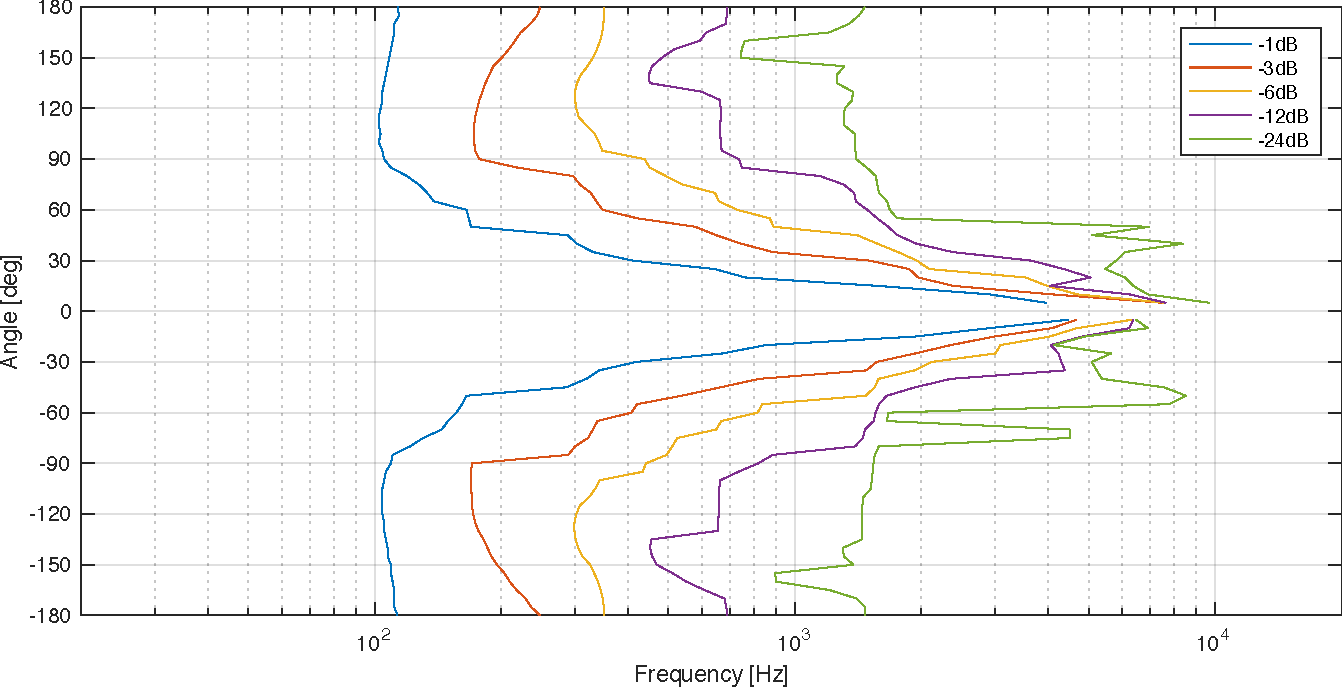
\includegraphics[width=1\textwidth]{beamwidth_off_4_5_cm.pdf}
	\caption{The figure shows the beamwidth to a specified \si{\decibel} change between the front measurement and a measurement from a given angle of the \gls{dut}. It find the first frequency where the \gls{spl} difference between front measurement and the measurement from the given angle is $n$\si{\decibel}, where $n$ is given in the figure. The \gls{dut} which correspond to this figure is a \citep{seas33}}
		\label{fig:beamwidth_offset_4.5_cm}
\end{figure}